\documentclass[a4paper,12pt]{article}
\usepackage[english]{babel}
\usepackage{graphicx}
\usepackage{amsfonts}
\usepackage{mathtools}
\usepackage{float}
\usepackage{makeidx}
\usepackage{bm}
\usepackage{listings}

\renewcommand{\topfraction}{.9}
\renewcommand{\bottomfraction}{.9}
\renewcommand{\textfraction}{.1}



\begin{document}
\begin{titlepage}

\title{MSO Lab Exercise III: Design and Refactoring}
\author{Chiel van Griethuysen (4014200) en In\`es Duits(3930971)}
\maketitle

\end{titlepage}

\newpage

\tableofcontents

\newpage

% % part 1
\section{Design – Comparison}

\subsection{Our original Design}
Our original Design looked like

\\
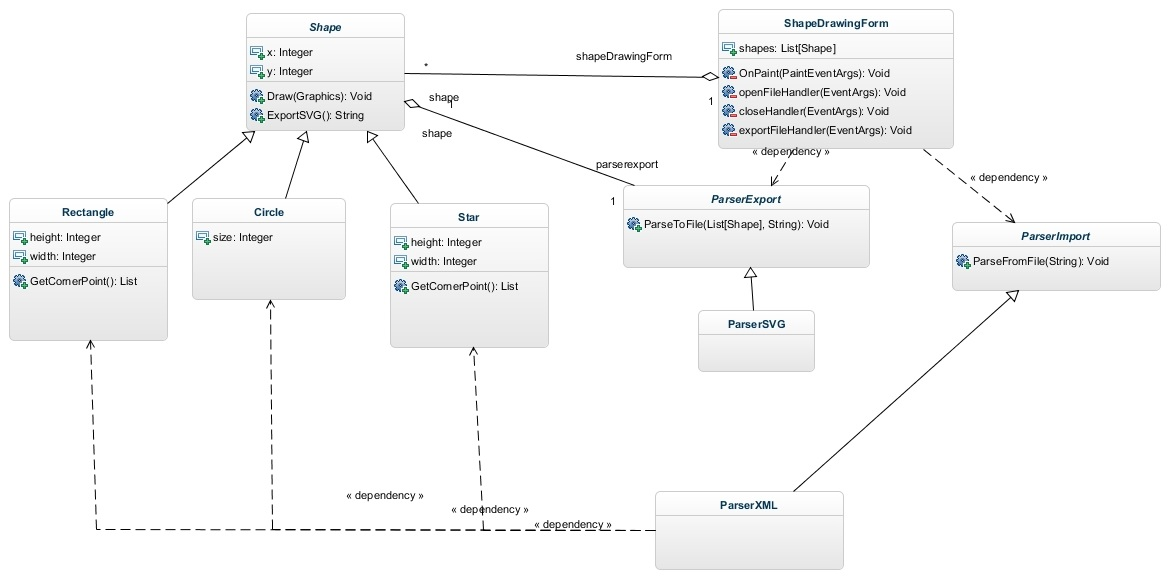
\includegraphics[scale=0.5]{diagram.jpg}
\\

You can see we kept the original Parser, but extend it to an abstract ParserImport, with only one subclass ParserXML. This so we can extend it for further use. We also decided to pulled some variables up in the abstract Shape class, the x and y coordinates which every shape should have.
\\
To solve the main problem, which was adding a way to draw and to export SVG code without duplicating code, we add a new abstract class ParserExport. This class would get a subclass, ParserSVG, which will handle exporting SVG code. We make a mistake by not really understanding how to apply the bridge pattern, so from that point we choose to give every Shape a new method. With that method, exportSVG, we would create a SVG code such that every object could represent itself. But this code would be much the same as the Draw method of each Shape. Our idea was a try, but we quite misunderstand the Parser concept. We thought the actual drawing should be not the same as SVG code, because Exporting and Importing is something different then actually drawing on the screen. Which, after rethought our design, it is not. But we still tried to split the Parser (our ParserExport) from the Visualisation (our ParserImport) although the names may be not good chosen. 
\\

% % Beter then?

So our Original Design is not quit better then the "extend the existing Shapes with a new method to produce SVG", because that is actually what we did. We created a new method for each shape, instead of creating new definitions to draw Lines en Circles.
\\
We were not planning on "copy-paste the existing visualization code into a new class and adapt it to produce SVG", but it could be that our solution used code which would look much like the existing graphic code, the original Draw method already had. 
\\
We try to not use any switch statement, to avoid "adding switch statements to the existing Shape classes to switch between drawing on screen or generating SVG files". So our original Design, although not good, did not use switch statements in the new found solution.


\subsection{Our Design}
We will add our Design before starting to code because we make a mistake which need to be solved first. The diagram looks much alike.

\\
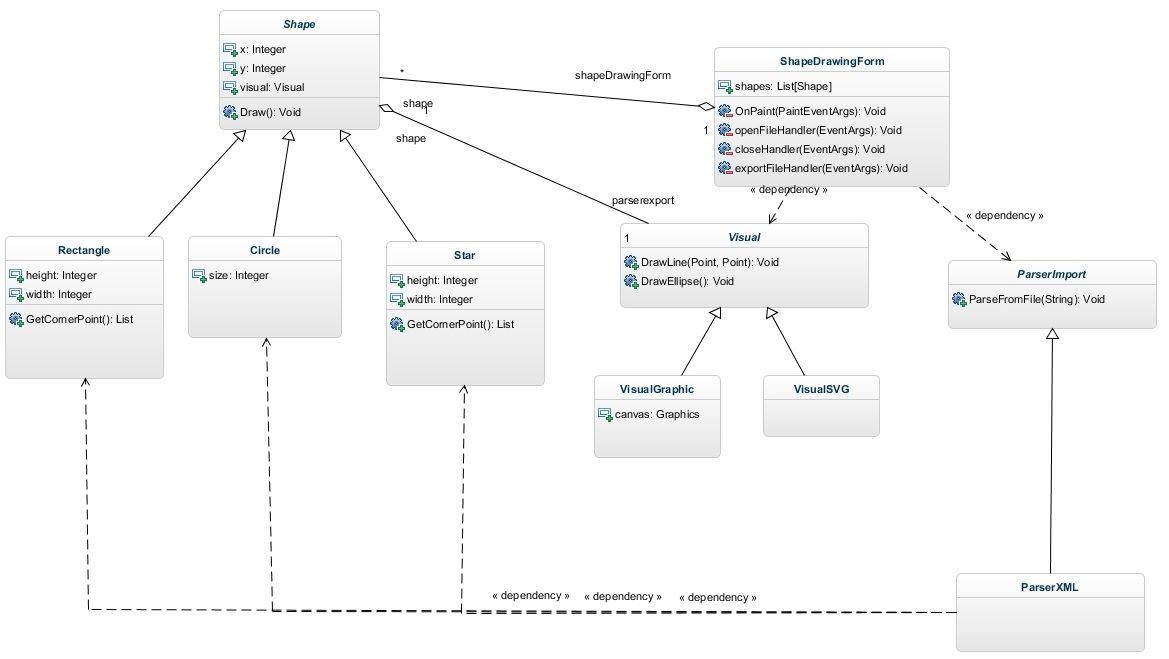
\includegraphics[scale=0.5]{diagramFinal.jpg}
\\

We still have the two abstract Parser methods, although we renamed the ParserExport to Visual, and his subclass, ParserSVG to VisualSVG. We add a new subclass to the renamed abstract Visual class, called VisualGraphics, which new task will be that what the Draw class of Shape did. The Visual class will get other methods, drawLine and drawCircle. After that we will recreate the Shape methods. We removed the ExportSVG method from the Shape class and we modify the Draw method. The Draw will now call the methods defined in Visual instead of the Graphics methods. The original code in Draw will be used to write the VisualGraphics class.
\\

% % Beter then?

We will try to implement this 'new' Design but it may change during the refactoring. By applying the Bridge pattern the good way, we avoid using switches or copy pasting the code. So now the "extend the existing Shapes with a new method to produce SVG" will not occur. Actually by adding a new Visual class, and giving every Shape a visual, there is no need in the future to change the Shape class in the event of a new export file type. Because we only have to add a new subclass to the Visual class, which will describe how the abstract defined methods (drawLine and drawCircle) of the Visual class should be handled.
\\
The new abstract Visual class also avoid "copy-pasting the existing visualization code into a new class and adapt it to produce SVG". By edeting the original Draw class to something which ask the Visual to draw instead, there is also no need to re-use the original Draw method in a new SVG draw class. We will give both the graphic and the SVG visual a way to implement the abstract methods of Visual and they both need a different output, so both a different code. But we do not have to tell both for SVG and for Graphics, that a Rectangle needs 4 lines. The Draw method of a Rectangle will tell the Visual to draw four lines, and the Draw method of the Star will tell the Visual to draw five lines. The Visual, independent from SVG or Graphic, will draw or four or five lines, not knowing that it is drawing a Rectangle or a Star.
\\
By giving each Shape his own (abstract) Visual, each Shape does not have to know to which type it is drawing. The ShapeDrawingForm class will make sure that every Shape has the right concrete Visual subclass, without the Shape actually care about it. The Shape class still will call the Draw method, independent from the Visual it has. So we avoid "adding switch statements to the existing Shape classes to switch between drawing on screen or generating SVG files.". The Shape does not know there are different Visuals to switch between, the ShapeDrawingForm will change to the right Visual depending on which event will occur.


% % part 2
\section{Implementation}

\subsection{Pull Up: Shapes}
%We see that the attributes in Rectangle, Circle and Star for the x and y position are all integers with the name x and y, and represent the appear position for this Shapes. Every new Shape should also need a x and y position. Therefore we can pull this attribute up to the abstract Shape class. Now we will compile the program to see if we didn't make a mistake.
The pulling up from the variables x and y, into the abstract Shapes, didn't give any trouble.


\subsection{Add Attribute}
%The original ShapeDrawingForm class suggest to have a Shapes. But because it is not shown in the original Design we introduce the attribute containing a List of Shapes. We need a way to store the shapes the ShapeDrawingForm class have to draw, and we think there was maybe another place where it was stored. But now we want to store it in a public attribute called shapes. It is useful because we need to give the shapes to the Parser class.
We looked at the code and we found that the current ShapeDrawingForm class already had a List of Shapes. So we did not need to add this List.

\subsection{Extract Variable: GetCornerPoints}
%We create the new methods, GetCornerPoints, in Star and Rectangle. For Star we will get the original code of his Draw function, transform it in a code to calculate the corner points and place it in the GetCornerPoints method. Then we will change draw method of Star, instead of using the complicated calculation, using the GetCornerPoints. Then we will do the same for Rectangle.
%Although the change is not big, testing and compiling the code on this point should be done. We need to know if the GetCornerPoints indeed calculate the correct corner points of a star and a rectangle. Also it is crucial that the draw methods of star and rectangle still draw the same star and rectangle. These two points should be tested.
In the original refactoring plan, the GetCornerPoints method should give back a List of Points. We changed this in a array of Points. The Points that will be return are in a specific order which we need to keep. We also add a lot of comments, to make clear how the calculation works for a maybe future change.
\subsubsection{Rectangle}
The subtraction from the four corners of a rectangle into a new function was not very hard.

\subsubsection{Star}
We already had a complicate code to calculate the Star Points. We used this code in the GetCornerPoints, which make the draw function itself look much less complicated.


\subsection{Introducing Abstract Class: ParserImport}
%The original program has only the class Parser, with the method ParseShapes. We will make it abstract and create the subclass ParseXML. 
We here made a new abstract ParserImport class, which is an abstract superclass for the original Parser.  It is not really necessary, to create an abstract class but it makes it easier to extend the code in the future.

\subsubsection{Rename Class and Push Down Method}
%The original Parser class already had the possibility to import a XML file with the method ParseShapes and thus we use that method in the subclass ParseXML. We choose to use this method but we will rename it to ParseFromFile, to make its purpose clearer. We will also define it already in the Abstract class, every new subclass (added in the future) should also have that method.
We renamed the Parser class to ParserXML, and made it a subclass from the ParserImport class. The re-arranging of the method went well, it was mostly a matter of renaming, the already exciting method could stay the same.


\subsubsection{Change Method in ShapeDrawingForm}
%We changed the name and the place of the original ParseShapes method. The ShapeDrawingForm classes called that method in his openFileHandler method. So we need to change the calling of the old ParseShape method into a calling for the new ParseFromFile method. Now it is very important that we test and compile the code. We did not really rewrite the original code from the method ParseShapes, but we need to make sure the reading from an XML file still works before we try to make the SVG export part. The class ShapeDrawingForm also need to call the right ParseFromFile method, instead of the old ParseShapes method which at this point doesn't exists any more.
We only need to change the call of the original Parser method into the new defined ParseFromFile method. Not a single problem occurred.


% % % % ABOND THE PLAN!!!  % % % % % % %
\subsection{Introducing Abstract Class: ParserExport -> Visual}
%We will introduce a new abstract class called the ParserExport with the method ParseToFile. Verwijzing Section 1
Here we will abandon the plan totally for the first time. As described in Section 1, our actually design of the new class which will generate SVG code need to be different, and we abandon the original 'ParserExport - plan'. We will create here, instead of the ParserExport, a abstract Visual class, with two methods: DrawLine and DrawCircle. This class will handle all the visualisations of the Shapes.

\subsubsection{Add new subclass: VisualSVG}
%Then we can add the subclass ParseSVG, which will implement a way to export every shape. The method ParseToFile will use the ExportSVG method for every Shape it needs to export, So there is no need for a switch in this method! 
We add the subclass VisualSVG, to the Visual class, which will implement the DrawCircle and DrawLine methods so that it will draw a circle or line in SVG code.

\subsubsection{Add new subclass: VisualGraphic}
We need to also visualize the original the Shapes in the program itself, like the original Draw method did. Therefore we create a new subclass under Visual, called VisualGraphic. We will define the methods DrawCircle and Drawline by using the original Draw method of each shape. This worked good, we only needed to copy past a few lines from two subclasses of Shape.

\subsubsection{Add attribute: Visual}
After defining the new visual code, we also need to give the Shape class a Visual. We add to the abstract Shape class an attribute, visual, so every created Shape have a Visual. This visual will be defined (or changed) depending on the type of Visual we need. This defining of changing will be done by the ShapeDrawingForm class.

\subsubsection{Change Method: Draw() in Shape}
The Draw method in every subclass of Shape needs to be changed. We will draw shapes using the defined visual instead of using the C\# oriented Graphics.

\subsubsection{Change Methods in ShapeDrawingForm}
%We need a way to call the new introduced method, ParseToFile. This will be done from the ShapeDrawingForm class if the user want to export the current file. Introducing a new method in ShapeDrawingForm called exportFileHandler, will handle the event if the user clicks export. Then we will have to compile and test the code! Because this is the point we introduces a whole new code, the export of the shapes into a SVG file. We need to make sure it works, and the shapes are exporting the right way.
We now have every class and method (changed), now they need to be called right methods in the ShapeDrawingForm class when an event happened. 
\\
The onPaint method do not need to change much, it still have to call the Draw method of each Shape. But now it also have to change the visual of each shape into VisualGraphic.
\\
The exportFileHandler method, need to export to a SVG file. We added the already excisting opening and closinig from a file. Write the basis syntax into a SVG file and added the shapes in a for loop. Here we also need to change the Visual of each Shape, before we can call the Draw method of each Shape.

\subsection{Add the Color}
We extending the our program so that it also could handle color's. This was not in our original (nor in our in section 1 described) design plan. We choose to add this feather. We had some deciding how to read the color from the XML file. You can save color like "Red" but also like "\#FF0000" and we want both to work. The visualisation of the Graphic draw part, worked almost immediately. But visualisation of the SVG file also had some trouble because of the 'how to describe' color problem, just like we had with the XML part.
\\
We created a solution by adding a new method, getRGBstring, which generated the needed SVG color values in string format. 

% % part 3
\section{Reflection}



\end{document}